\section{IEC \glspl{FB}}
\thispagestyle{fancy}



%Skriv OM:
%Programmering av IEC Blokker (MB,MA,SBE,SBV) 
%+ fb blokker (fbTimer, fbAnalougeAlarm, fbCAC)
%- Til appendiks, Heile kode for t.d. fbTimer, fbCAC osv

% Skrive litt om blokka sin funksjonalitet
% Korleis me brukte blokkene i programmet.

\textbf{Skrive om at alle IEC blokkene har alarmutgang og feilmeldings(int) for seinare alarmhandtering, tilrettelagt for feilhandtering}\newline
Vi gjore eit utval av blokker basert på dei komponentane vi hadde identifiserte i annlegget.
For å laga eit robust program valde vi og fokusere på: \gls{MA}, \gls{MB}, \gls{SBE} og \gls{SBV}.
Sjølv om blokkene kunne verke noko overkvalifiserte valde vi likevel å ha dei med, da nokon av tilleggsfunksjonane eventuelt kunne nyttast seinare
og at det gav oss ein klar retning å arbeide mot.

\gls{IEC} har sentrale begreper som vi ynskjer å utdjupe nærmare. Grunna mangel på gode norske begreper 
og for å forhindre forvirring har vi valgt å beskrive begrepa slik dei er definert i normen.

\begin{itemize}
    \item \textbf{Lock:} Action overruling any other signal while being true
    \item \textbf{Force:} Action overruling any other signal
    \item \textbf{Disable Transition:} Transistion high/low function not avaliable
    \item \textbf{Blocking:} Prevention of certain functions or operations 
    \item \textbf{Suppression:} Disable alarm annunciation as well as any associated automatic actions
\end{itemize}

Alle blokkene som er designet etter IEC PAS 63131, har alle handtering av feil med utgang som indikerer om det er noko feil, og ein eigen utgang med ein numerisk feilkode for identifisering av korleis feilkode blokka gir. 
Desse funksjonane er veldig viktig i videre arbeid mot feilhandtering og alarmliste. 

\subsection{Monitor Analogue}
\gls{MA} funksjonsblokka (Legg til appendix her) er brukt for skalering, visning, overvåking og alarmhandtering av analoge inngangsvariablar i ein prosess.
Funksjonsblokka inneheld 'supression' og 'blocking' funksjonalitet.

funksjonsblokka er brukt i programmet for å overvåke analoge trykknivågivarar samt å skalere og vise desse som ein fyllingsgrad i prosent.

\begin{figure}[htbp]
    \centering
    \begin{subfigure}[b]{0.45\textwidth}
        \centering
        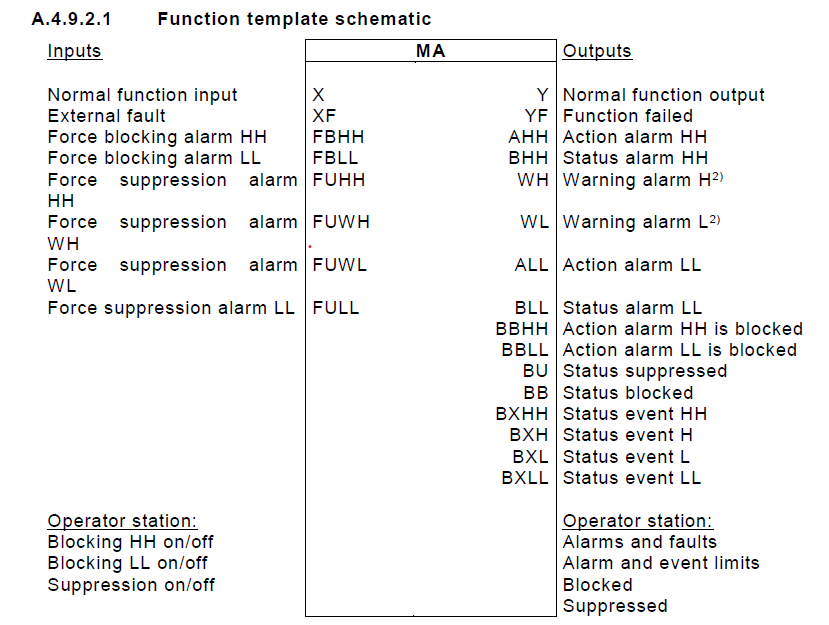
\includegraphics[width=1\textwidth]{Bilder/MABlokkIEC.png}
        \caption{IEC}\label{fig:Monitor Analogue blokk IEC}
    \end{subfigure}
    \hfill
    \begin{subfigure}[b]{0.45\textwidth}
        \centering
        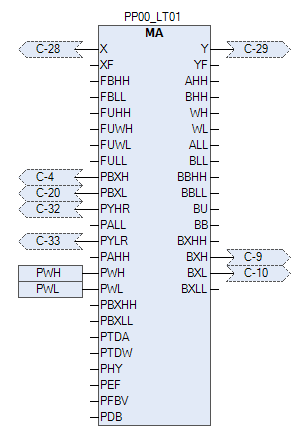
\includegraphics[width=0.7\textwidth]{Bilder/MABlokkIProgrammet.png}
        \caption{Bruk i programmet}\label{fig:Monitor Analogue blokk i programmet}
    \end{subfigure}
    \caption{Monitor Analogue}\label{fig:Monitor Analogue}
\end{figure}
\newpage

\subsection{Monitor Binary}
\gls{MB} \gls{FB} (Legg til appendix her) blir brukt til automatisk overvåking, alarmhandtering, framvising og latching av binære prosess variablar.
\gls{FB} inkluderer alarm suppression og blokkerings funksjonalitet. Den har moglegheit for invertering av 
inngangssignal og moglegheit for tids forseinking av utgangssignal via parameter.

Funksjonsblokka er brukt i programmet for å overvaka alle digitale nivåfølerar i prosessen.


\begin{figure}[htbp]
    \centering
    \begin{subfigure}[b]{0.45\textwidth}
        \centering
        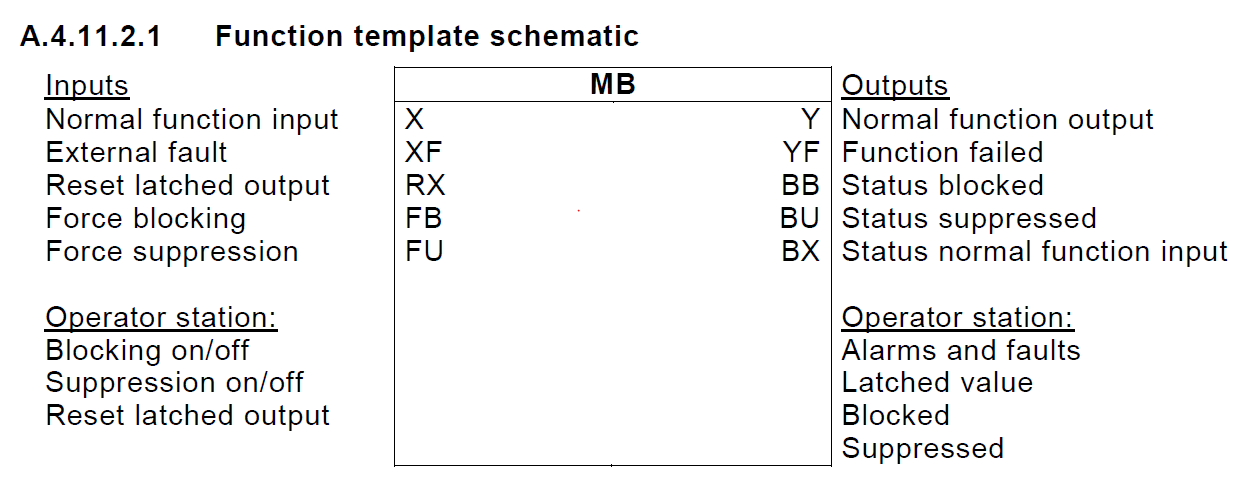
\includegraphics[width=1\textwidth]{Bilder/MBBlokkIEC.png}
        \caption{IEC}\label{fig:Monitor Binary blokk IEC}
    \end{subfigure}
    \hfill
    \begin{subfigure}[b]{0.45\textwidth}
        \centering
        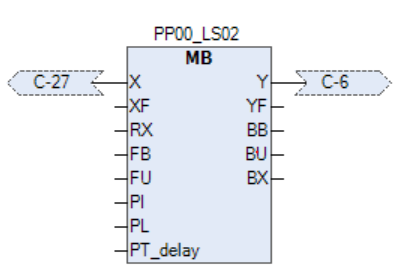
\includegraphics[width=0.7\textwidth]{Bilder/MBBlokkIProgrammet.png}
        \caption{Bruk i programmet}\label{fig:Monitor Binary blokk i programmet}
    \end{subfigure}
    \caption{Monitor Binary}\label{fig:Monitor Binary}
\end{figure}

\newpage

\subsection{Switch Binary Valve}

\gls{SBV} \gls{FB} (Legg til appendix her) skal brukast til binær av/på kontroll av eit straumningselement ved å endra straumen av medium (varme eller væske). 
Typisk komponentar som styrast er bl.a. ventilar og spjeld.
\gls{FB} er i dette programmet brukt til og styre ventilar.

\gls{FB} styrer ventilen ved hjelp av dei binære inngangane XH og XL.
Desse inngangane styrer ein utgang Y, som sender opne/stenge-kommando(høg/låg) til ventilaktivatoren.
Alternativt kan dei pulsmodulerte utgangane YH og YL kan også nyttast.

\gls{FB} har også inngongar XGH og XGL som gjer tilbakemelding om ventilen er heilt open eller stengd,
som då bekrefter ventilen sin posisjon.

\textbf{Kontrollfunksjonane i \gls{FB} inkluderar:}
\begin{itemize}
    \item Generering av feilstatus (YF) om det oppstår ein intern eller ekstern feil.
    \item Blokka set utgangen Y i samsvar med parameter når feil blir oppdaga.
    \item Blokka set utgangen Y basert på tilbakemelding i "outside mode" når ingen eksterne inngangar blir brukte (XOH/XOL).
\end{itemize}

Funksjonsblokka inkluderar alarm suppression, blocking, safeguarding og transition funksjonalitet.

\begin{figure}[htbp]
    \centering
    \begin{subfigure}[b]{0.45\textwidth}
        \centering
        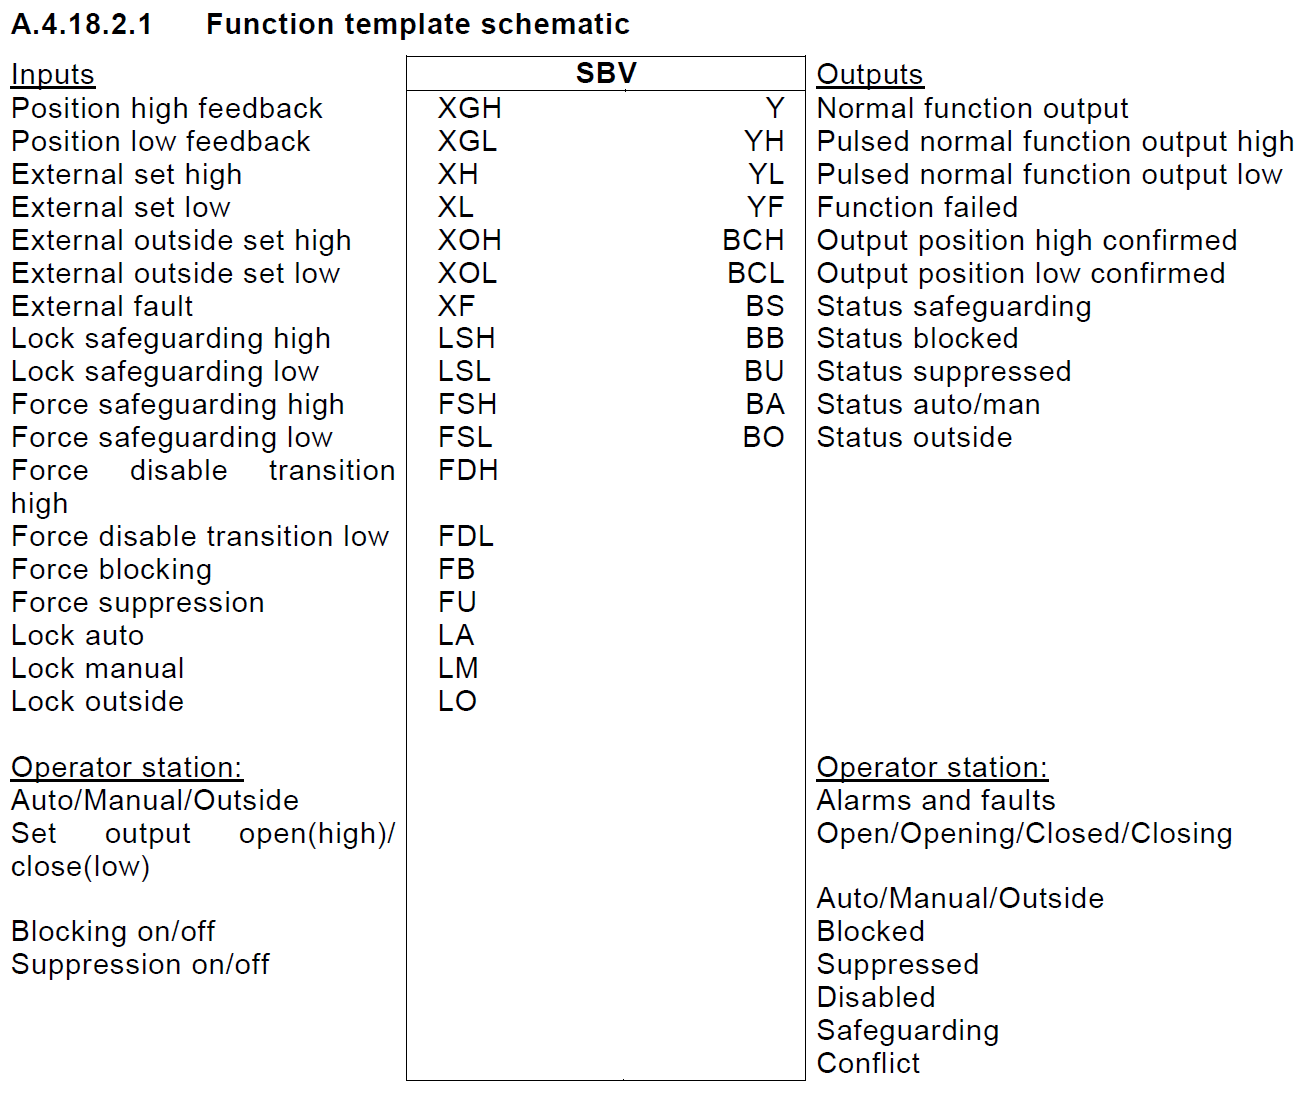
\includegraphics[width=1\textwidth]{Bilder/SBVBlokkIEC.png}
        \caption{IEC}\label{fig:Switch Binary Value blokk IEC}
    \end{subfigure}
    \hfill
    \begin{subfigure}[b]{0.45\textwidth}
        \centering
        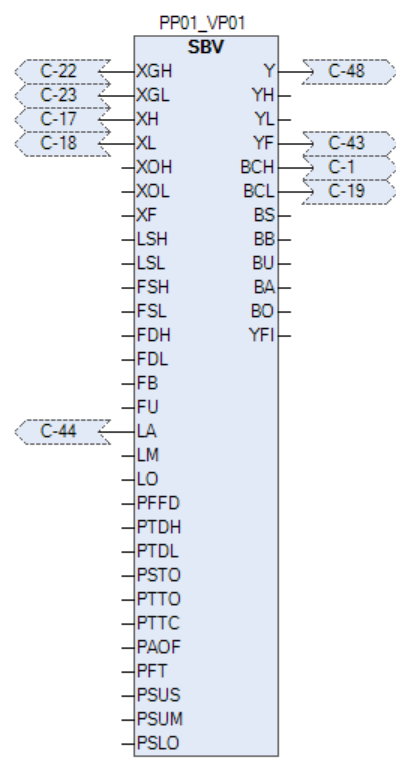
\includegraphics[width=0.5\textwidth]{Bilder/SBVBlokkIProgrammet.png}
        \caption{Bruk i programmet}\label{fig:Switch Binary Value blokk i programmet}
    \end{subfigure}
    \caption{Switch Binary Value}\label{fig:Switch Binary Value}
\end{figure}

\newpage

\subsection{Switch Binary Eletrical}

\gls{FB} (Legg til appendix her) blir brukt for binærkontroll (av/på) kontroll av straumningselement for elektrisitet, varme eller væske. Det
kontrollerte komponenten er av typen motor, pumpe, varmeelement, vifte etc.

\gls{FB} beskriver korleis ein kontrollarar ein komponent, som tl.d. Motor, pumpe, varmeelement eller ei vifte.
Det er utgangen Y, som sender ein opne/stenge kommando(høg/lav) til komponenten. Blokka har fleire funksjonar, der den
tar utgangen og samanliknar med tilbakemelding (XGH) som gjer korrekt (BCL/BCH) status. Den genererer også ein feil status på
(YF) om ein har ein ekstern feil inn(XF).

\gls{FB} inkluderer alarm suppression, blocking, safeguarding og transition funksjonalitet.

\begin{figure}[htbp]
    \centering
    \begin{subfigure}[b]{0.45\textwidth}
        \centering
        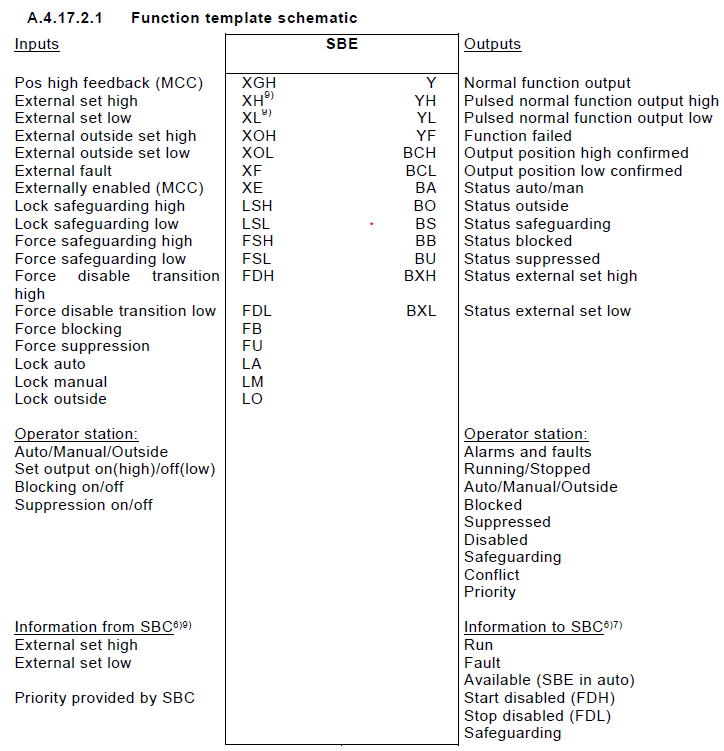
\includegraphics[width=1\textwidth]{Bilder/SBEBlokkIEC.png}
        \caption{IEC}\label{fig:Switch Binary Eletrical blokk IEC}
    \end{subfigure}
    \hfill
    \begin{subfigure}[b]{0.45\textwidth}
        \centering
        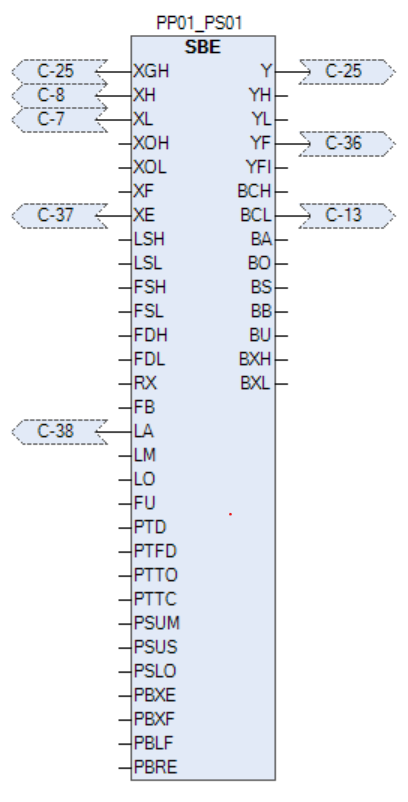
\includegraphics[width=0.5\textwidth]{Bilder/SBEBlokkIProgrammet.png}
        \caption{Bruk i programmet}\label{fig:Switch Binary Eletrical blokk i programmet}
    \end{subfigure}
    \caption{Switch Binary Eletrical}\label{fig:Switch Binary Eletrical}
\end{figure}

\newpage

%\begin{figure}[htbp]
%    \centering
%    \begin{subfigure}[b]{0.45\textwidth}
%        \centering
%        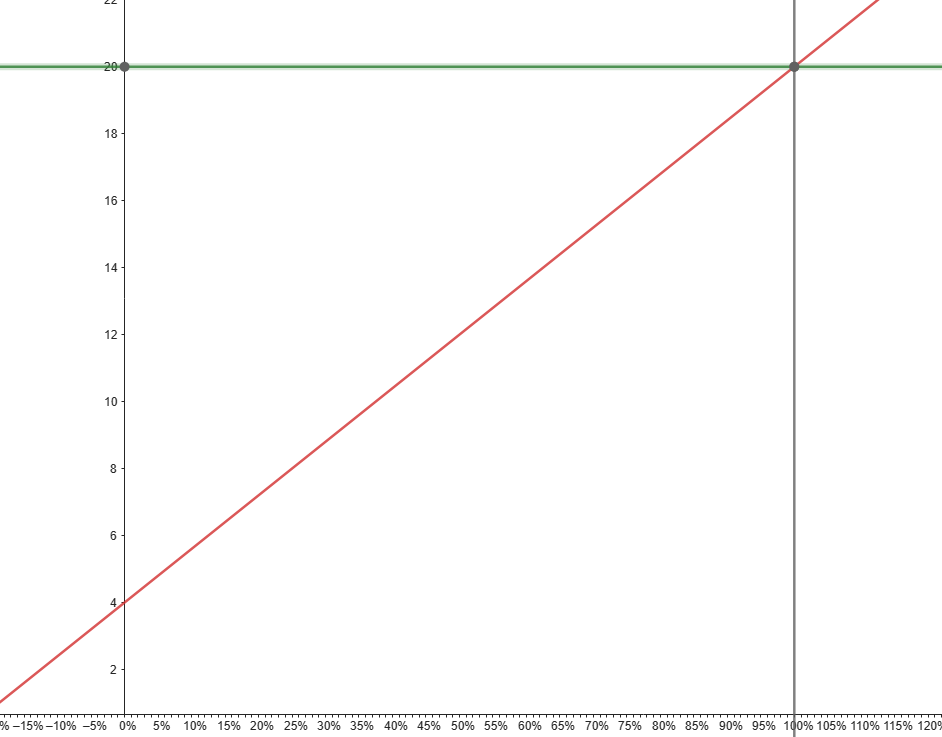
\includegraphics[width=1\textwidth]{Bilder/4_20mA_Scaling.png}
%        \caption{Skalering av mA mot prosent}\label{fig:Skalering av mA mot prosent}
%    \end{subfigure}
%    \hfill
%    \begin{subfigure}[b]{0.45\textwidth}
%        \centering
%        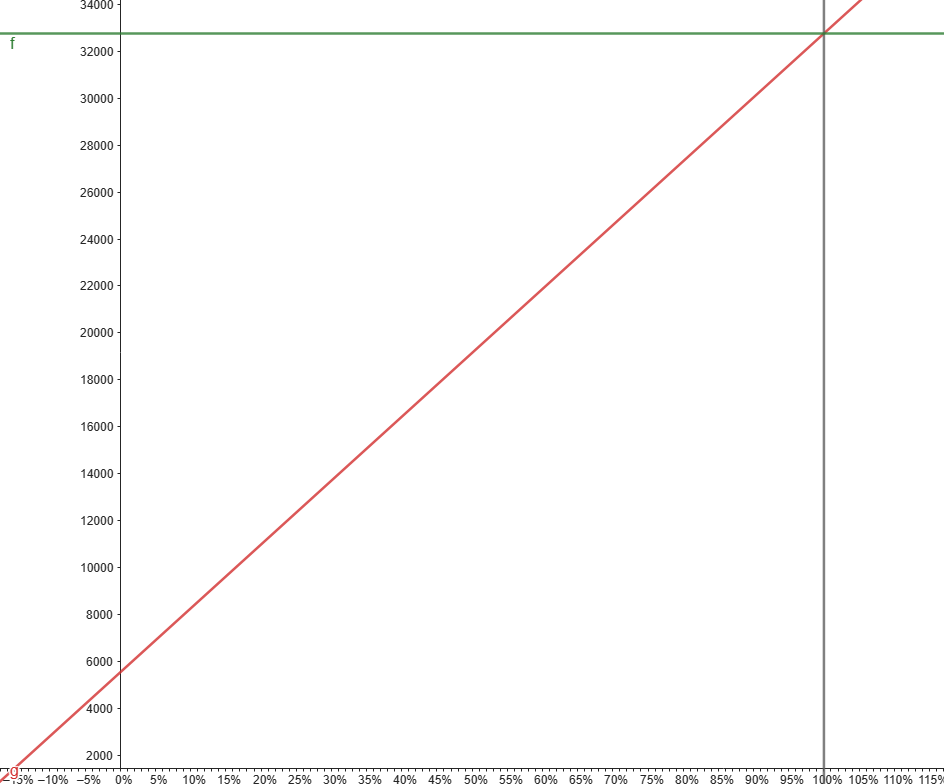
\includegraphics[width=0.95\textwidth]{Bilder/27327_prosent_Scaling.png}
%        \caption{Skalering av prosent til verdi}\label{fig:Skalering av prosent til verdi}
%    \end{subfigure}
%    \caption{Dei forskjellige skaleringane av inngangssignal}\label{fig:Skalering av prosent til verdi}
%\end{figure}


